\section{Theorie}
Die Strahlung, die in diesem Versuch untersucht wird, ist die $gamma$-Strahlung. Diese elektromagnetische Strahlung ist höherenergetisch als Röntgenstrahlung mit Energien von mindestens $\SI{100}{keV}$. Sie entsteht bei Übergängen zwischen Anregungszuständen im Atomkern. $\gamma$-Strahlung ist nicht direkt beobachtbar, sie muss also erst mit Materie wechselwirken. Die Produkte dieser Wechselwirkung (im Normalfall Elektronen) sind dann beobachtbar.
\subsection{Wechselwirkung von $\gamma$-Strahlung mit Materie}
In diesem Versuch werden die drei häufigsten Prozesse betrachtet: der Photoeffekt, der Compton-Effekt und die Paarbildung.
\subsubsection{Photoeffekt}
Beim Photoeffekt löst das Photon ein Elektron aus der Atomhülle eines Atoms heraus und wird dabei selbst absorbiert. Ein Teil der Energie des Photon wird dabei für die Austrittsarbeit $W_\text{A}$ verwendet, den Rest erhält das Elektron als kinetische Energie. Dieses Elektron kann nun detektiert werden. Da zur Impulserhaltung während des Vorgangs ein weiteres Teilchen benötigt wird, werden meist Elektronen aus inneren Schalen gelöst, sodass der zusätzliche Impuls an den Atomkern abgegeben werden kann. Den freien Platz in der Atomhülle nimmt nun ein Elektron aus einer höheren Schale ein, dass dabei Röntgenstrahlung oder ein Augerelektron abgibt. In beiden Fällen kann die Energie schlussendlich vom Detektor gemessen werden, sodass die gesamte Energie des ursprünglichen $\gamma$-Quants nachgewiesen werden kann.

\subsubsection{Comptoneffekt}
Beim Comptoneffekt streut das $\gamma$-Photon an einem quasifreien Elektron, also einem Elektron der äußeren Atomhülle. Dabei wird ein Teil der Energie des Photons auf das Elektron übertragen, welches in einem Winkel $\theta$ zur ursprünglichen Bahn des Photons abgelenkt wird. Das Photon wird dabei um den Winkel $-\theta$ gestreut und besitzt die verringerte Energie $E_\gamma'$. Die Energie des Elektrons nach dem Stoß lässt sich mit \cref{eq:compton} berechnen.

\begin{equation}
	E_e = E_\gamma \left( 1-\frac{1}{1 + \frac{E_\gamma}{m_ec^2}\left( 1-\cos\left(\theta\right)\right)}\right)
	\label{eq:compton}
\end{equation}

Die übertragene Energie ist also vom Winkel abhängig. Während bei einem Winkel von $0$° keine Energie übertragen wird, ist die Energie bei einem Winkel von $180$° maximal. Unter welchem Winkel die Teilchen streuen ist dabei statistisch verteilt. Wenn also nur gestreutes Elektron detektiert wird, kann daraus ohne Information über den Winkel keine Information über die ursprüngliche Energie des $\gamma$-Quants gewonnen werden. Wenn aber sehr viele Photonen detektiert werden entsteht ein kontinuierliches Spektrum mit einer deutlichen Kante bei der Energie, die das Elektron bei einem Stoß um $180$° erhalten hat, der Comptonkante. Daraus sind Rückschlüsse auf die Energie des Photons möglich.

\subsubsection{Paarbildung}
Der dritte auftretende Effekt nennt sich Paarbildung. Hierbei erzeugt das Photon ein Elektron-Positron-Paar und annihiliert dabei. Die Energie muss mindestens $\SI{1022}{keV}$ betragen, da diese als Ruhemasse der entstehenden Teilchen benötigt wird. Der Rest geht in kinetische Energie der Teilchen über. Dieser Prozess kann nur in Materie stattfinden, da ein weiterer Reaktionspartner (meistens ein Atomkern) benötigt wird, um den überschüssigen Impuls aufzunehmen. Das Elektron kann in diesem Zustand bereits detektiert werden, das Positron allerdings bildet zuerst mit einem anderen Elektron zusammen Positronium. Dieser Zustand zerfällt allerdings nach einiger Zeit und erzeugt so einige Photonen (die Anzahl ist abhängig von den Spins der beiden Teilchen). Diese können nun wiederum über einen der beschriebenen Effekte Elektronen erzeugen, die detektiert werden können. Die Wahrscheinlichkeit, dass einer der oben genannten Prozesse auftritt, steigt mit zunehmender Ladungszahl des Absorbermaterials. Daher werden für die Detektoren schwere Elemente wie z.B. Blei verwendet. Außerdem ist die Wahrscheinlichkeit abhängig von der Energie des Photons. Dieser Zusammenhang ist in \cref{streuung} dargestellt.

\begin{figure}[h!]
	\centering
	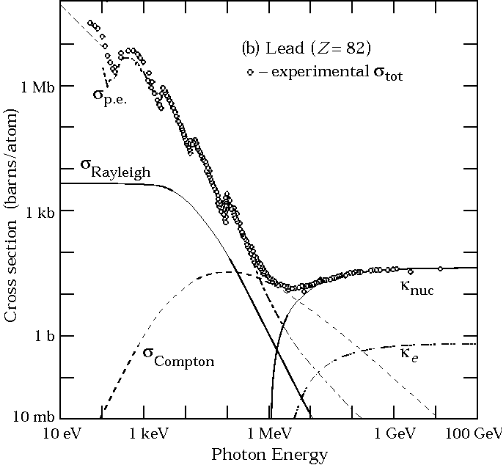
\includegraphics[width=0.9\textwidth]{streuung.PNG}
	\caption{Dargestellt ist der Wirkungsquerschnitt der einzelnen Effekte in Abhängigkeit von der Energie des Photons in Blei. Bei niedrigen Energien dominiert der Photoeffekt, bei mittleren der Comptoneffekt, bei hohen die Paarbildung. Die Kanten beim Photoeffekt kommen zustande, da genau bei dieser Energie das Photon genug Energie hat, um Elektronen aus einer weiteren, tieferen Schale zu lösen.}
	\label{streuung}
\end{figure}

Bei niedrigen Energien überwiegt der Photoeffekt, bei mittleren Energien zwischen $\SI{300}{keV}$ und $\SI{7}{MeV}$ überwiegt der Comptoneffekt, anschließend die Paarbildung.

\subsection{Detektoren}
In diesem Versuch werden zwei verschiedene Detektorentypen verwendet: Ein Halbleiterdetektor und ein Szintillationsdetektor. der Halbleiterdetektor besteht aus mit Lithium dotiertem Germanium, der Szintillator ist ein Natriumjodid-Kristall, der mit Thallium aktiviert ist. Beide Detektoren wandeln die auftreffende $\gamma$-Strahlung in Elektronen um,  die dann mithilfe verschiedener Bauteile in ein messbares Signal umgewandelt werden können, allerdings auf unterschiedliche Weise. Beide Möglichkeiten werden im folgenden kurz vorgestellt.

\subsubsection{Halbleiterdetektor}
In Halbleitern wird durch auftreffende Photonen ein Elektron-Loch-Paar erzeugt. Dies kann, wenn an den Halbleiter eine Spannung anliegt, abgezogen und gemessen werden. Allerdings wäre hierfür ein hochreiner intrinsischer Halbleiter nötig, da sonst Blindsträme auftreten, die eine gute Messung unmöglich machen. Alternativ wird daher ein sogenannter intrinsic-Kristall verwendet. Bei diesem werden in einen p-dotierten Halbleiter Lithiumatome gegeben, die als n-Dotierung wirken und so die p-Dotierung ausgleichen. Diese Kristalle haben sehr ähnliche Eigenschaften wie intrinsische Halbleiter. So können Sperrschichten mit einer Größe von mehreren Zentimetern zu erzeugen. Die Breite der Sperrschicht ist dabei proportional zur Quadratwurzel der angelegten Spannung. Diese Kristalle werden als pn-Übergang in Sperrrichtung betrieben. Trifft nun ein Photon auf den Kristall, entstehen Elektron-Loch-Paare, die sofort durch die anliegende Spannung getrennt werden und so am rekombinieren gehindert werden. Diese Teilchen erzeugen durch Stöße weitere Elektron-Loch-Paare. Durch die anliegende Hochspannung werden die Ladungsträger aus dem Halbleiter abgezogen und können als Strom gemessen werden.

\subsubsection{Szintillationsdetektor}
Ein Szintillationsdetektor besteht aus zwei Komponenten, dem Szintillator und dem Photomultiplier. Im Szintillator wird die hochenergetische $\gamma$-Strahlung in niederenergetisches sichtbares Licht umgewandelt. Organische Szintillatoren nutzen zur Umwandlung der Strahlung Molekülanregungen, in anorganischen Szintillatoren entstehen das sichtbare Licht durch Übergänge in den Bändern des Kristalls. Durch die auftreffende Strahlung wird ein Elektron-Loch-Paar erzeugt, das anschließend rekombiniert und ein Photon mit der Energie der Bandlücke abgibt. Da dieses Photon an anderen Atomen des Szintillators wieder ein Elektron-Loch-Paar erzeugen und daher den Kristall nicht verlassen würde, werden sogenannte Aktivatoren in den Kristall gegeben. Dies sind Atome mit anderer Bandlücke. Die so entstehenden Photonen erzeugen also mit geringerer Wahrscheinlichkeit wieder ein Elektron-Loch-Paar und können den Kristall verlassen. Anschließend gelangen die Photonen in den Photomultiplier. Dort schlagen die Photonen an einer Kathode Elektronen aus. Diese werden nun durch ein elektrisches Feld auf Dynoden gelenkt, an denen sie nun Sekundärelektronen erzeugen. Diese wiederum erzeugen an der nächsten Dynode weitere Sekundärelektronen, sodass am Ende ein messbares Signal vorliegt.

\subsection{Methoden und Aufbau}
Um die detektierten Elektronen in ein messbares Signal zu verwandeln, werden noch einige Bauteile benötigt. Zuerst wird das Signal von einem Vorverstärker auf eine Spannung von einigen $100$ mV verstärkt, um es über ein Kabel übertragen zu können. Dabei bekommt es die Form eines exponentiellen Abfalls. Anschließend wird es von einem Hauptverstärker weiter verstärkt und zu einem gaußförmigen Signal geformt, sodass es von den weiteren Bauteilen verarbeitet werden kann. Nun wird das Signal von einem Analog-Digital-Wandler digitalisiert. Zuletzt sortiert ein Multi-Channel-Analyzer die Pulse nach ihrer Energie in verschiedene Kanäle ein. Der hier verwendete MCA besitzt etwa $8000$ verschiedene Channels. Dieser wurde am Anfang mit der Probe, bei der die höchsten Energien zu erwarten waren, so eingestellt, dass alle Channels verwendet werden. So kann die bestmögliche Auflösung sichergestellt werden.

\subsection{$\gamma$-Spektrum}
Die Signale, die auf die verschiedenen Channels des MCA verteilt wurden, können nun am Computer dargestellt werden. Signale, die auf denselben Channel geschickt wurden, werden aufsummiert, sodass die Anzahl der Ereignisse für verschiedene Energien des detektierten Elektrons dargestellt wird. Da die Energie des detektierten Elektrons proportional zur Energie des $\gamma$-Quants ist, können so Rückschlüsse die $\gamma$-Strahlung gezogen werden. Das erwartete Spektrum, idealisiert, ohne Rauschen, ist in \cref{idealized_spectrum} dargestellt.

\begin{figure}
	\centering
	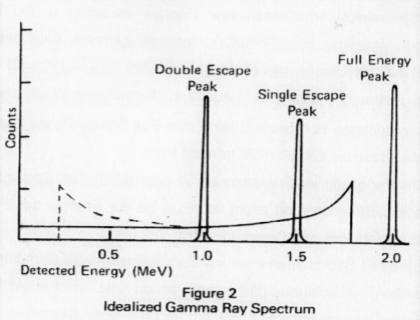
\includegraphics[width=0.8\textwidth]{gammaray.png}
	\caption{Idealisiertes Spektrum der $\gamma$-Strahlung. Ganz rechts der Full Energy Peak, der durch den Photoeffekt und bei der Paarbildung, wenn beide durch Zerstrahlung des Positrons entstandenen Photonen noch im Detektor reagieren. Daneben der Single Escape Peak, der auftritt, wenn eines der vom Positron erzeugten Photonen nicht mehr im Detektor reagiert und ganz links der Double Escape Peak, für den Fall, dass beide Photonen nicht reagieren. Zwischen Single Escape Peak und Full Energy Peak ist die Comptonkante zu sehen, die bei Compton-Streuung um $180$° auftritt. Bei niedrigeren Energien ist daneben die kontinuierliche Verteilung für die Streuung unter anderen Winkeln sichtbar}
	\label{idealized_spectrum}
\end{figure}

Der Hauptpeak ist der sogenannte Full Energy Peak. Er tritt auf, wenn die gesamte Energie des $\gamma$-Quants im Detektor gemessen wird. Dies ist vor allem der Fall beim Photoeffekt. Er tritt außerdem beim Comptoneffekt auf, wenn sowohl das gestreute Photon als auch das Elektron detektiert werden. Bei der Paarbildung zerstrahlt nach kurzer Zeit das Positronium und erzeugt dabei meist zwei Photonen. Wenn diese beide noch im Detektor durch andere Wechselwirkungen Elektronen erzeugen, die vom Detektor erfasst werden, trägt auch dieser Effekt um Full Energy Peak bei. Wenn jedoch eines der Photonen nicht mehr im Detektor wechselwirkt, trägt dieser Vorgang zum Single Escape Peak bei. Dieser ist zum Full Energy Peak um $\SI{511}{keV}$ zu tieferer Energie verschoben. Entkommen beide Photonen aus dem Detektor entsteht der Double Escape Peak, welcher um $\SI{1022}{keV}$ zum Full Energy Peak verschoben ist. Da beim Comptoneffekt ein kontinuierliches Spektrum an Elektronen, abhängig vom Streuwinkel, entsteht, ist dieser Effekt auch als kontinuierliche Verteilung zwischen den Energien $0$ und $E_\text{max}$ sichtbar. Ab $E_\text{max}$ tritt dieser Effekt nicht mehr auf, daher ist an dieser Stelle die bereits erwähnte Comptonkante zu sehen.

Es werden aber auch noch andere Elektronenenergien gemessen, um die das Ergebnis am Ende bereinigt werden muss. Der sogenannte Backscatteruntergrund entsteht durch Compton-Streuung der $\gamma$-Quanten am Abschirmmaterial. Dabei kann ein Photon mit Energien zwischen $E_\text{min}$ und $E_\gamma$ zurück in den Detektor gelangen und dort zum Signal beitragen. So entsteht eine weitere kontinuierliche Verteilung mit Energien zwischen $E_\text{min}$ und $E_\gamma$. Außerdem können durch Photoeffekt am Abschirmmaterial weitere Peaks entstehen, die genau den Energieabständen zwischen zwei Schalen in der Atomhülle dieser Elemente entsprechen.


\section{Auswertung}
\subsection{Kalibration}
Zunächst muss die Kalibrierung bestimmt werden. Dies ist nötig, da die verschiedenen Zählungen in "Channels" unterteilt wurden. Um die Messungen allerdings sinnvoll zu verwenden, ist es nötig die korrespondierenden Energien, zu den jeweiligen Channels zu kennen. Dafür wird zunächst die Messung der $^{22}$Na in \cref{Kali} betrachtet.

\begin{figure}[ht]
	\centering
	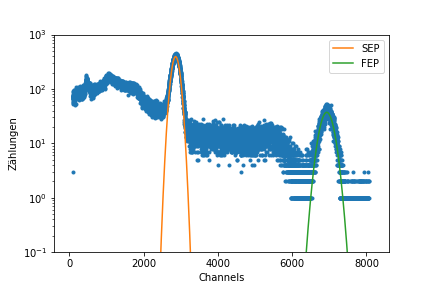
\includegraphics[scale=0.8]{na.png}
	\caption{Messung des $^{22}$Na Spektrums mithilfe des Szintillators.}
	\label{Kali}
\end{figure}

in der Messung sind deutlich zwei Peaks zu sehen, einen Full Energy Peak(FEP) und einen Single Escape Peak(SEP). Da die Literaturwerte der beiden Peaks mit $E_{FEP} = \SI{1274,5}{keV}$ und $E_{SEP} = \SI{511}{keV}$ bekannt sind und außerdem ein linearer Zusammenhang zwischen den Channels und den zugehörigen Energien besteht, kann eine Umrechnung stattfinden.
Das passiert mit der Formel:
\begin{equation}
E = m \cdot Ch + E_{0},
\end{equation}  
wobei
\begin{equation}
m = \frac{E_{FEP} - E_{SEP}}{Ch_{FEP} - Ch_{SEP}}
\end{equation}
und 
\begin{equation}
E_{0} = E_{FEP} - m \cdot Ch_{FEP}
\end{equation}
mit $Ch$ dem jeweilig zugehörigem Channel. Für den Szintillator ergibt das eine Umrechnung von $m = \SI{0,18769 \pm 0,00007}{\frac{keV}{Ch}}$ und $E_{0} = \SI{-26,5 \pm 0,56}{keV}$. Die Umrechnung für den Halbleiter funktioniert analog und ergibt einen Faktor von $m = \SI{0,169868 \pm 0,000002}{\frac{keV}{Ch}}$ und $E_{0} = \SI{0,01 \pm 0,01}{keV}$. 



\subsection{Unsicherheiten}
Innerhalb der Fehlerrechnung wurden zwei Fehlerquellen angenommen. Der erste Fehler ist vom Fit-Programm fityk ausgegeben worden. Dieser hat für die Werte eine Genauigkeit angegeben. Der zweite Fehler ist durch die Kalibrierung hinein gekommen. Alle weiteren Fehler wurden mittels Fehlerfortpflanzung ermittelt.


\subsection{$\gamma$-Spektren}

\subsubsection{$^{22}$Na Szintillator}
In \cref{na_sz} ist das mithilfe des Szintillators aufgenommene Spektrum der $^{22}$Na-Quelle zu sehen. 

\begin{figure}[ht]
	\centering
	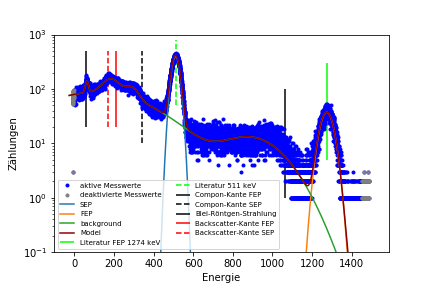
\includegraphics[scale=0.8]{na_sz_.png}
	\caption{$^{22}$Na Szintillator Spektrums auf die korrekten Energien kalibriert.}
	\label{na_sz}
\end{figure}

Da die Kalibrierung mit diesem Spektrum stattgefunden hat, ist es nicht möglich mit  damit die Genauigkeit der Peaks selbst zu diskutieren. Allerdings passen die ausgerechneten Compton- und Backscatterkanten gut mit den im Spektrum sichtbaren Kanten überein. Ein weiterer Peak bei etwa 70 keV lässt sich allerdings nur über die Funktionsweise des Szintillators erklären, der mit Blei abgeschirmt wird. Durch diese Abschirmung kann Röntgenstrahlung entstehen, wenn ein Elektron in der innersten Schale durch einen Stoß mit einem Photon oder freiem Elektron entfernt wird, weshalb ein Elektron aus einer höheren Schale in die niedrigere Schale springen muss, wobei es Energie abgibt. Es ist also die K-Linie von Blei dort zu sehen.




\subsubsection{$^{60}$Co Szintillator}
Als nächstes wird das Co-Spektrum in \cref{co_sz} betrachtet. Die Probe hat zwei verschiedene Übergänge, die auch beide bei deutlich zu sehen sind. Allerdings ist ihr Mittelpunkt mit $E_{FEP1} = \SI{1176,1 \pm 0,7}{keV}$ und $E_{FEP2} = \SI{1335,8 \pm 0,8}{keV}$ jeweils etwa 3keV größer als der Literaturwert. Trotzdem passen die Compton und - Backscatterkanten wieder gut mit dem sichtbaren Spektrum überein, wobei insbesondere interessant ist, dass die beiden Backscatterkanten übereinander liegen und damit einen größeren Peak als sonst erzeugen.



\begin{figure}[ht]
	\centering
	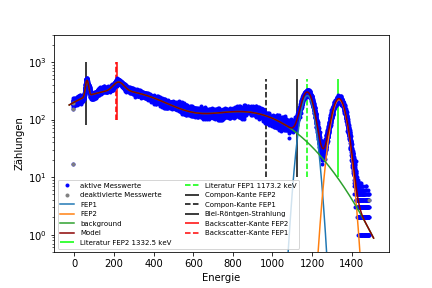
\includegraphics[scale=0.8]{co_sz_.png}
	\caption{$^{60}$Co Spektrum mit einem Szintillator aufgenommen.}
	\label{co_sz}
\end{figure}

\subsubsection{$^{137}$Cs Szintillator}
Danach wird das Spektrum der $^{137}$Cs-Probe betrachtet, das in \cref{cs_sz} zu sehen ist. In diesem Fall gibt es nur einen Übergang und damit auch nur einen Full Energy Peak. Allerdings ist auch hier wieder der Mittelpunkt dieses Peaks mit $E_{FEP1} = \SI{663,5 \pm 0,6}{keV}$ etwa 2keV größer als der Literaturwert. Allerdings passen die Compton- und Backscatterkante wieder gut ins Spektrum rein.



\begin{figure}[ht]
	\centering
	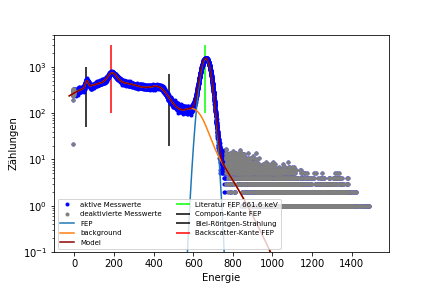
\includegraphics[scale=0.8]{cs_sz_.png}
	\caption{$^{60}$Cs Spektrum mit einem Szintillator aufgenommen.}
	\label{cs_sz}
\end{figure}



\subsubsection{Mischquelle Szintillator}

\begin{figure}[ht]
	\centering
	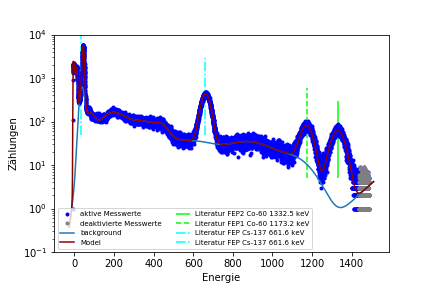
\includegraphics[scale=0.8]{Mischquelle_sz_.png}
	\caption{Mischquelle mit einem Szintillator aufgenommen.}
	\label{Mischquelle_sz}
\end{figure}


Daraufhin wird eine Mischquelle betrachtet, die aus mehreren Elementen besteht und zugeordnet werden sollen. Die beiden Elemente die sich ohne Probleme zuordnen lassen sind $^{137}$Cs und $^{60}$Co. Die Peaks im gemessenen Spektrum befinden sich für das Cobalt bei $E = \SI{662,2 \pm 0,7}{keV}$ und für Cäsium bei $E = \SI{1172,8 \pm 0,9}{keV}$ und $E = \SI{1329,3 \pm 1}{keV}$, wobei nur der größte $^{137}$Cs Peak etwas vom Literaturwert abweicht. Es lassen sich allerdings noch vier weitere Peaks im niedrigeren Energiebereich erkennen, die schwieriger zuzuordnen sind. Der Größte davon liegt bei $E = \SI{44,8 \pm 0,6}{keV}$ und könnte am ehesten mit weiteren möglichen Übergängen von $^{137}$Cs erklärt werden, die bei $\SI{31,8}{keV}$ und $\SI{32.2}{keV}$ stattfinden. Die drei kleineren Peaks, die ineinander übergehen befinden sich nach der Messung zwischen 9,6 und -5,5keV, was offensichtlich keinen Sinn ergibt, da negative Energien nicht auftreten können. Allerdings handelt es sich dabei höchstwahrscheinlich wieder um Röntgenstrahlung und die einzelnen Peaks korrespondieren mit der $K_{\alpha}$ bis $K_{\gamma}$ Linie. Allerdings wird dabei deutlich, dass die Annahmen der Linearität zwischen Channels und Energie, bei der Kalibrierung im niedrigen Energiebereich nicht mehr gilt und dann zu deutlich größeren Fehlern führt.








\subsubsection{$^{22}$Na Halbleiterdetektor}

\begin{figure}[ht]
	\centering
	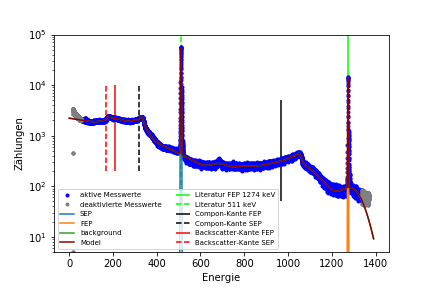
\includegraphics[scale=0.8]{na_pn_.png}
	\caption{$^{22}$Na Spektrum mit einem Halbleiterdetektor aufgenommen.}
	\label{na_pn}
\end{figure}

Die Kalibrierung hat auch für den Halbleiterdetektor wieder über die $^{22}$Na Probe stattgefunden, weshalb die Peaks natürlich wieder mit den Literaturwerten übereinstimmen. Im Vergleich zu der Szintillatormessung in \cref{na_sz} fällt allerdings auf, dass die Peaks eine sehr viele schmaler sind und damit eine geringere Energieunschärfe besitzen. Außerdem werden beim Halbleiterdetektor keine Röntgenstrahlung mehr festgestellt, da kein Blei als Abschirmung vorhanden ist. Ungewöhnlich ist auch, dass die Comptonkante des FEP fast 100keV von der Kante im Bild entfernt ist.



\newpage
\subsubsection{$^{60}$Co Halbleiterdetektor}


\begin{figure}[ht]
	\centering
	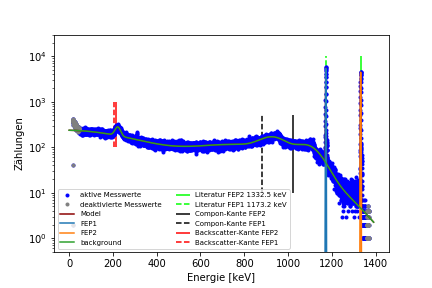
\includegraphics[scale=0.8]{co_pn_.png}
	\caption{$^{60}$Co Spektrum mit einem Halbleiterdetektor aufgenommen}
	\label{co_pn}
\end{figure}


Als nächstes ist die $^{60}$Co probe, die mit einem Halbleiterdetektor gemessen wurde, in \cref{co_pn} zu sehen. Die beiden FEPs befinden sich bei $E_{FEP1} = \SI{1172,6 \pm 0,1}{keV}$ und $E_{FEP2} = \SI{1331,7 \pm 0,1}{keV}$, was jeweils etwa 1keV kleiner als der Literaturwert ist. Beide Comptonkanten sind außerdem wieder kleiner als die gemessen Kanten im Spektrum. 

\newpage
\subsubsection{$^{137}$Cs Halbleiterdetektor}

In \cref{cs_pn} ist das Spektrum vom Cäsium durch den Halbleiterdetektor aufgenommen
zu sehen. Der FEP befindet sich bei $\SI{661,5 \pm 0,1}{keV}$, was mit dem Literaturwert übereinstimmt. Die Comptonkante und Backscatterkante sind wieder etwas zu klein, liegen allerdings grundsätzlich im richtigen Bereich.


\begin{figure}[ht]
	\centering
	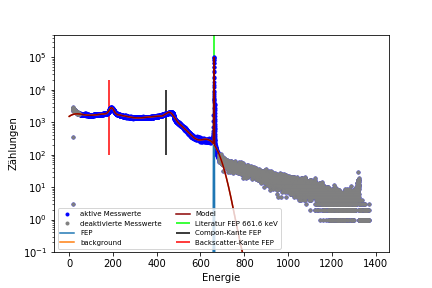
\includegraphics[scale=0.8]{cs_pn_.png}
	\caption{$^{137}$Cs Spektrum mit einem Halbleiterdetektor aufgenommen}
	\label{cs_pn}
\end{figure}

\newpage
\subsection{Erz Halbleiterdetektor}
Als letztes soll ein vorher unbekanntes Erz untersucht werden und einer der drei natürlichen Zerfallsreihe zugewiesen werden.  Das Spektrum ist in \cref{Erz_pn} zu sehen. Alle Elemente die im Bild eingezeichnet sind, sind Teil der Uran-238 Reihe und stimmen, außer bei sehr großen und sehr niedrigen Energien, immer gut mit den eingezeichneten Peaks überein. Für die beiden anderen Zerfallsreihen waren keine solche Übereinstimmungen zu sehen. Somit kann davon ausgegangen werden, dass es sich um diese Zerfallsreihe handelt.

\begin{figure}[ht]
	\centering
	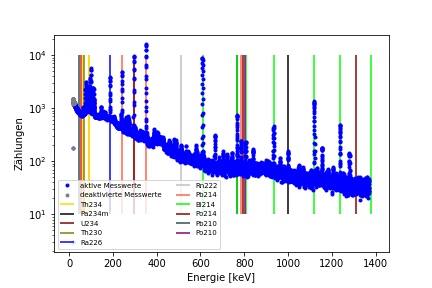
\includegraphics[scale=0.8]{Erz_pn_.png}
	\caption{$^{137}$Cs Spektrum mit einem Halbleiterdetektor aufgenommen}
	\label{Erz_pn}
\end{figure}





\newpage
\subsection{Diskussion}
Insgesamt passen die Ergebnisse ziemlich gut, die Peaks unterscheiden sich meistens nur wenige keV vom Literaturwert  und auch Compton- und Backscatterkanten konnten immer gut zugeordnet werden. Außerdem ließen sich sowohl die Mischquelle als auch das Erz ohne Problem zuordnen. Allerdings waren die Unsicherheit fast immer zu klein, wobei zwei grundsätzliche Fehler der Grund sein könnten. Erstens wurde die Unsicherheit der Detektoren überhaupt nicht betrachtet und wenn diese einen signifikanten Teil der Unsicherheit ausmacht, kann das dazu führen , dass die Unsicherheiten zu klein sind. Ein andere Möglichkeit ist, dass die Unsicherheiten der Gauß-Fits und damit auch der Kalibration zu klein waren.


\subsection{Detektoreigenschaften}
\subsubsection{ Relative Abweichung von den Referenzwerten.}
In \cref{ee} ist die relatve Differenz von gemessener zur Referenzenergie gegen die Referenzenergie aufgetragen. Die Fehlerbalken wurden durch die Fehler, welche das Programm fityk ausgerechnet hat mittels Fehlerfortpflanzung berechnet.Es ist zu erkennen, dass die relativen Abweichungen der gemessenen Werte vom Halbleiterdetektor näher an den Referenzwerten liegen, als die Werte die mittels des Szintillators berechnet wurden. Dies kann bei drei Werten erkannt werden. Die anderen beiden Werte liefern unabhängig von ihrern Fehlern dieselben Ergebnisse. Hier ist anzufügen, dass die Fehlerbalken mittels des Szintillators größer ausgefallen sind, als die Fehlerbalken des Halbleiter Detektors.
\begin{figure}[h!]
	\centering
	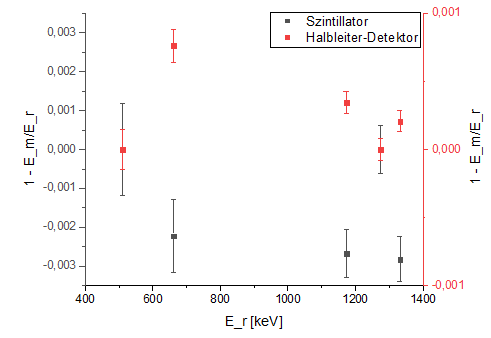
\includegraphics[width=0.9\textwidth]{1minEdurchE.png}
	\caption{Auf der $y$-Achse ist die relative Differenz zwischen gemessenen Energien und auf der $x$-Achse die Referenzenergie aufgetragen.}
	\label{ee}
\end{figure}
\subsubsection{Energieauflösung}
Als weiteren Vergleichspunkt wird die Energieauflösung ($\Delta E$) der beiden Detektoren berechnet.
Die Energieauflösung ($\Delta E = \frac{\sigma}{E}$) beschreibt die Energiebreite des Peaks zur jeweiligen Energie. Dabei wurde die Breite des Gaußpeaks ($\sigma$) über das Full Width at Half Maximum bestimmt.
In \cref{sig} sieht man beide Energieauflösungen aufgetragen. Die Unsicherheiten sind zu klein, als dass diese im Diagramm zu erkennen wären.
Die Nullniveaus der beiden Achsen sind unterschiedlich aufgetragen. Das Nullniveau des Szintillators ist nach oben verschoben, wohingegen das Nullniveau des Halbleiter-Detektors nach unten verschoben ist. Anhand der Grafik kann abgelesen werden, dass die Energieauflösung beider Detektoren mit zunehmender Energie zunimmt.
Weiterhin sind die Skalierungen der Achsen nicht gleich, sodass das Auflösungsvermögen des Halbleiterdetektors weniger um das Nullniveau schwankt, als dass des Szintillators. Somit besitzt der Halbleiter-Detektor eine bessere Auflösung als der Szintillator.
Beim Halbleiter-Detektor befindet sich das Auflösungsvermögen im Bereich von $10^{-4}$ bis $10^{-3}$, wohingegen sich das Auflösungsvermögen beim Szintillator in einem Bereich von $10^{-2}$ bis $2*10^{-2}$ befindet.
Dies veranlasst uns dazu, die Erzprobe nicht mit dem Szintillator, sondern mit dem Halbleiter-Detektor aufzunehmen.
\begin{figure}[h!]
	\centering
	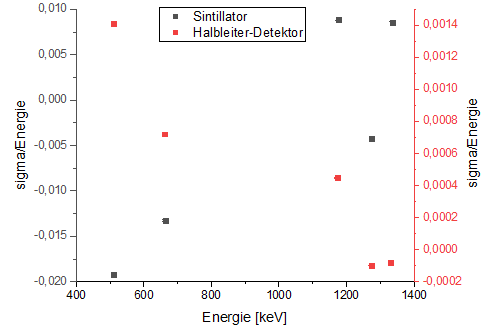
\includegraphics[width=0.9\textwidth]{sigma.png}
	\caption{}
	\label{sig}
\end{figure}
\subsubsection{Mittlere Ionisationsenergie}
Die Ionisationsenergie ($I = \frac{E}{N}$), wobei N die Anzahl von Zählungen ist, kann mittels der Energieauflösung und der Annahme, dass $\sigma$ Poisson verteilt ist zu $I = \frac{\sigma^2}{E}$ umgeformt werden.
In \cref{sig2} ist die Ionisierungsenergie bezüglich der Energie aufgetragen. Aufgrund der unterschiedlichen Skalierung der Achsen für Szintillator und Halbleiter-Detektor ist zu erkennen, dass die Ionisierungsenergien beim Halbleiter-Detektor geringer sind als beim Szintillator. Die Ionisationsenergie des Szintillators liegen bei maximal $0,2$ keV, wohingegen die Ionisationsenergien beim Halbleiter-Detektor maximal bei $0,001$ keV liegen.
\begin{figure}[h!]
	\centering
	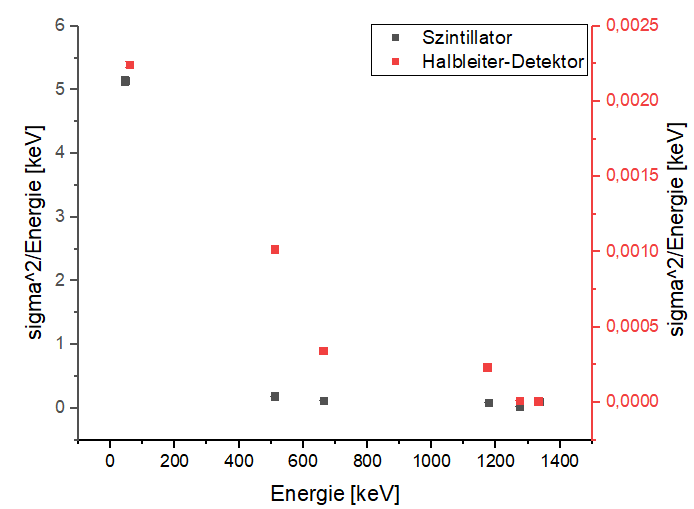
\includegraphics[width=0.9\textwidth]{sigma2.png}
	\caption{Mittlere Ionisationsenergie für beide Detektoren in Abhängigkeit der Energie}
	\label{sig2}
\end{figure}
\subsubsection{Effizienz}
Die Effizienz ist ein Maß für den Anteil der detektierten Photonen von der Gesamtzahl theoretisch nachweisbarer Photonen. Dieser Parameter ist von verschiedenen Parametern abhängig. Die Effizienz ist von der Aktivität der Stoffe und von geometrischen Eigenschaften, wie vom Raumwinkel, abhängig. Somit kann die Effizienz vom Szintillator nicht mit der Effizienz vom Halbleiter-Detektor verglichen werden. Ebenfalls kann die Effizienz nicht von unterschiedlichen Quellen verglichen werden. So kann nur die Effizienz der Mischquelle am Szintillator oder Halbleiter-Detektor untersucht werden. In diesem Versuch wurde die Effizienz nur an dem Szintillator untersucht. Die Effizienz ist definiert als, 
\begin{align}
	\epsilon = \frac{\frac{Area}{A}}{|\frac{Area}{A}|}
\end{align}
Die Normierung ist von dem Stoff höchster Aktivität pro Fläche zu nehmen.
In \cref{eff} ist zu sehen, dass die Effizienz im niederenergetischen Bereich maximal ist, wohingegen die Effizienz mit zunehmender Energie abfällt. Da der Wirkungsquerschnitt im niederenergetischen Bereich am größten ist, ist die Effizienz heir ebenfalls am größten. Der Wirkungsquerschnitt fällt mit zunehmender Energie ab, sodass hier die Effizienz abnimmt.
\begin{figure}[h!]
	\centering
	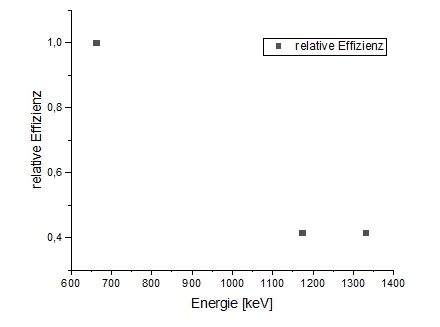
\includegraphics[width=0.9\textwidth]{Effizienz.png}
	\caption{}
	\label{eff}
\end{figure}

